\documentclass[12pt]{report}
\usepackage[utf8]{inputenc}
\usepackage[russian]{babel}
%\usepackage[14pt]{extsizes}
\usepackage{listings}
\usepackage{graphicx}
\usepackage{amsmath,amsfonts,amssymb,amsthm,mathtools} 
\usepackage{pgfplots}
\usepackage{filecontents}
\usepackage{indentfirst}
\usepackage{eucal}
\usepackage{amsmath}
\usepackage{enumitem}
\frenchspacing

\usepackage{indentfirst} % Красная строка


%\usetikzlibrary{datavisualization}
%\usetikzlibrary{datavisualization.formats.functions}

\usepackage{amsmath}




% Для листинга кода:
\lstset{ %
language=c++,                 % выбор языка для подсветки (здесь это С)
basicstyle=\small\sffamily, % размер и начертание шрифта для подсветки кода
numbers=left,               % где поставить нумерацию строк (слева\справа)
numberstyle=\tiny,           % размер шрифта для номеров строк
stepnumber=1,                   % размер шага между двумя номерами строк
numbersep=5pt,                % как далеко отстоят номера строк от подсвечиваемого кода
showspaces=false,            % показывать или нет пробелы специальными отступами
showstringspaces=false,      % показывать или нет пробелы в строках
showtabs=false,             % показывать или нет табуляцию в строках
frame=single,              % рисовать рамку вокруг кода
tabsize=2,                 % размер табуляции по умолчанию равен 2 пробелам
captionpos=t,              % позиция заголовка вверху [t] или внизу [b] 
breaklines=true,           % автоматически переносить строки (да\нет)
breakatwhitespace=false, % переносить строки только если есть пробел
escapeinside={\#*}{*)}   % если нужно добавить комментарии в коде
}

\usepackage[left=2cm,right=2cm, top=2cm,bottom=2cm,bindingoffset=0cm]{geometry}
% Для измененных титулов глав:
\usepackage{titlesec, blindtext, color} % подключаем нужные пакеты
\definecolor{gray75}{gray}{0.75} % определяем цвет
\newcommand{\hsp}{\hspace{20pt}} % длина линии в 20pt
% titleformat определяет стиль
\titleformat{\chapter}[hang]{\Huge\bfseries}{\thechapter\hsp\textcolor{gray75}{|}\hsp}{0pt}{\Huge\bfseries}


% plot
\usepackage{pgfplots}
\usepackage{filecontents}
\usetikzlibrary{datavisualization}
\usetikzlibrary{datavisualization.formats.functions}

\begin{document}
%\def\chaptername{} % убирает "Глава"
\thispagestyle{empty}
\begin{titlepage}
	\noindent \begin{minipage}{0.15\textwidth}
	
\includegraphics[width=\linewidth]{b_logo}
	\end{minipage}
	\noindent\begin{minipage}{0.9\textwidth}\centering
		\textbf{Министерство науки и высшего образования Российской Федерации}\\
		\textbf{Федеральное государственное бюджетное образовательное учреждение высшего образования}\\
		\textbf{~~~«Московский государственный технический университет имени Н.Э.~Баумана}\\
		\textbf{(национальный исследовательский университет)»}\\
		\textbf{(МГТУ им. Н.Э.~Баумана)}
	\end{minipage}
	
	\noindent\rule{18cm}{3pt}
	\newline\newline
	\noindent ФАКУЛЬТЕТ $\underline{\text{«Информатика и системы управления»}}$ \newline\newline
	\noindent КАФЕДРА $\underline{\text{«Программное обеспечение ЭВМ и информационные технологии»}}$\newline\newline\newline\newline\newline
	
	
	\begin{center}
		\noindent\begin{minipage}{1.3\textwidth}\centering
			\Large\textbf{  Отчёт по лабораторной работе №2}\newline
			\textbf{по дисциплине "Анализ алгоритмов"}\newline\newline
		\end{minipage}
	\end{center}
	
	\noindent\textbf{Тема} $\underline{\text{Умножение матриц}}$\newline\newline
	\noindent\textbf{Студент} $\underline{\text{Варламова Е.А.}}$\newline\newline
	\noindent\textbf{Группа} $\underline{\text{ИУ7-51Б}}$\newline\newline
	\noindent\textbf{Оценка (баллы)} $\underline{\text{~~~~~~~~~~~~~~~~~~~~~~~~~~~}}$\newline\newline
	\noindent\textbf{Преподаватели} $\underline{\text{Волкова Л.Л.}}$\newline\newline\newline
	
	\begin{center}
		\vfill
		Москва~---~\the\year
		~г.
	\end{center}
\end{titlepage}
\newpage
\setcounter{page}{2}
\tableofcontents

\chapter*{Введение}
\addcontentsline{toc}{chapter}{Введение}
Умножение матриц — это один из базовых алгоритмов, который широко применяется в численных методах, в частности, в машинном обучении, в компьютерной графике. Именно поэтому важно, чтобы алгоритм был максимально эффективен по затрачиваемым ресурсам. Так, \textbf{целью} данной работы является изучение алгоритмов умножения матриц, в частности: обычный алгоритм, алгоритм Винограда и оптимизированный алгоритм Винограда. 

Для достижения поставленной цели необходимо решить следующие задачи.
\begin{enumerate}
	\item Изучение двух алгоритмов умножения матриц: обычного и алгоритма Винограда.
	\item Разработка оптимизированного алгоритма умножения матриц.
	\item Реализация трёх алгоритмов умножения матриц: обычного, алгоритма Винограда и оптимизированного алгоритма Винограда.
	\item Сравнительный анализ трудоёмкости алгоритмов на основе расчетов в выбранной модели вычислений.
	\item Сравнительный анализ алгоритмов на основе экспериментальных данных.
\end{enumerate}

\chapter{Аналитическая часть}
В данном разделе рассматриваются два алгоритма умножения матриц - стандартный и Винограда. При этом предполагается, что количество столбцов первой умножаемой матрицы совпадает с количеством строк второй матрицы.
\section{Стандартный алгоритм}

Пусть даны две прямоугольные матрицы
\begin{equation}
	A_{rs} = \begin{pmatrix}
		a_{11} & a_{12} & \ldots & a_{1s}\\
		a_{21} & a_{22} & \ldots & a_{2s}\\
		\vdots & \vdots & \ddots & \vdots\\
		a_{r1} & a_{r2} & \ldots & a_{rs}
	\end{pmatrix},
	\quad
		B_{sc} = \begin{pmatrix}
		b_{11} & b_{12} & \ldots & b_{1c}\\
		b_{21} & b_{22} & \ldots & b_{2c}\\
		\vdots & \vdots & \ddots & \vdots\\
		b_{s1} & b_{s2} & \ldots & b_{sc}
	\end{pmatrix},
\end{equation}
тогда матрица $C$
\begin{equation}
	C_{rc} = \begin{pmatrix}
		c_{11} & c_{12} & \ldots & c_{1c}\\
		c_{21} & c_{22} & \ldots & c_{2c}\\
		\vdots & \vdots & \ddots & \vdots\\
		c_{r1} & c_{r2} & \ldots & c_{rc}
	\end{pmatrix},
\end{equation}
где
\begin{equation}
	\label{eq:M}
	c_{ij} =
		\sum_{t=1}^{s} a_{it}b_{tj} \quad (i=\overline{1,r}; j=\overline{1,c})
\end{equation}
будет называться произведением матриц $A$ и $B$. Стандартный алгоритм реализует данную формулу.

\section{Алгоритм Винограда}

Если посмотреть на результат умножения двух матриц, то видно, что каждый элемент в нем представляет собой скалярное произведение соответствующих строки и столбца исходных матриц.
Можно заметить также, что такое умножение допускает предварительную обработку, позволяющую часть работы выполнить заранее.

Рассмотрим два вектора $V = (v_1, v_2, v_3, v_4)$ и $W = (w_1, w_2, w_3, w_4)$.
Их скалярное произведение равно: $V \cdot W = v_1w_1 + v_2w_2 + v_3w_3 + v_4w_4$, что эквивалентно (\ref{for:new}):
\begin{equation}
	\label{for:new}
		V \cdot W = (v_1 + w_2)(v_2 + w_1) + (v_3 + w_4)(v_4 + w_3) - v_1v_2 - v_3v_4 - w_1w_2 - w_3w_4.
\end{equation}
Несмотря на то, что второе выражение требует вычисления большего количества операций, чем стандартный алгоритм: вместо четырёх умножений - шесть, а вместо трёх сложений - десять, выражение в правой части последнего равенства допускает предварительную обработку: его части можно вычислить заранее и запомнить для каждой строки первой матрицы и для каждого столбца второй, что позволит для каждого элемента выполнять лишь два умножения и пять сложений, складывая затем только лишь с 2 предварительно посчитанными суммами соседних элементов текущих строк и столбцов.
Из-за того, что операция сложения быстрее операции умножения в ЭВМ, на практике алгоритм должен работать быстрее стандартного.

Формула \ref{for:new} подходит лишь для того случая, когда длина векторов чётная. Соответственно, если количество столбцов первой матрицы (или количество строк второй) нечётное, то требуется сделать дополнительный проход по результирующей матрице и добавить в её элементы недостающие произведения.


\section{Вывод}
	В данном разделе были рассмотрены алгоритмы классического умножения матриц и алгоритм Винограда. Было выявлено, что алгоритм Винограда отличается от стандартного наличием предварительной обработки строк и столбцов, что позволяет сократить количество умножений, а значит ускорить алгоритм. 
\clearpage

\chapter{Конструкторская часть}

В данном разделе разрабатываются схемы алгоритмов, описанных в аналитическом разделе, а также даётся оценка трудоёмкости этих алгоритмов.
\section{Схемы алгоритмов}

На рисунках  \ref{fig:base}, \ref{fig:grapes} и \ref{fig:grapesOpt} приведены схемы стандартного алгоритма умножения матриц и алгоритма Винограда (обычного и оптимизированного) соответственно. Предполагается, что размеры первой матрицы (n1, m1), а второй - (n2, m2).

Алгоритм Винограда оптимизируется следующим образом.
\begin{enumerate}
\item Cокращается количество умножений в основном цикле и циклах предварительной обработки строк и столбцов.
\item Дополнительный цикл, работающий при нечётном количестве столбцов первой матрицы (строк второй), заменяется на условный оператор, помещённый в основной цикл.
\end{enumerate}

\begin{figure}[h!p]
	\centering
	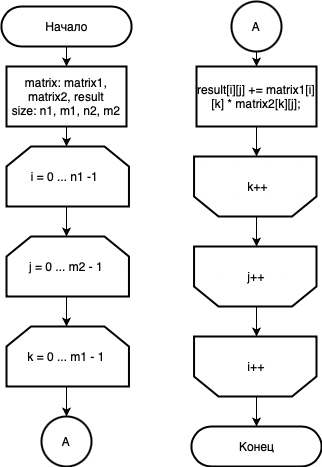
\includegraphics[scale = 0.55]{base.drawio.png}
	\caption{Схема стандартного алгоритма умножения матриц}
	\label{fig:base}
\end{figure}
\begin{figure}[h!p]
	\centering
	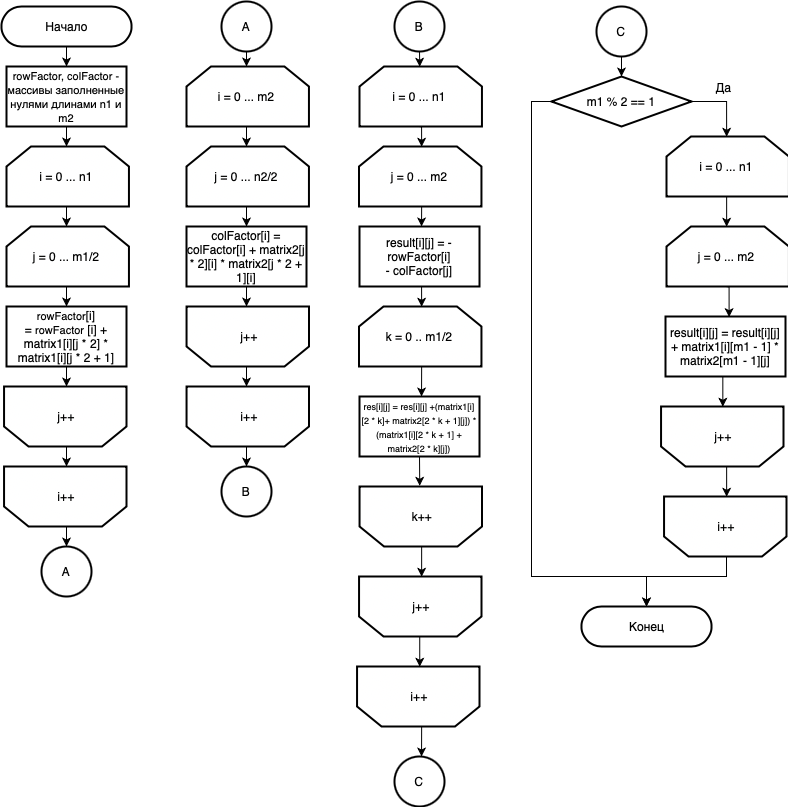
\includegraphics[scale = 0.65]{vin.drawio.png}
	\caption{Схема алгоритма Винограда}
	\label{fig:grapes}
\end{figure}
\begin{figure}[h!p]\label{vinOptScheme}
	\centering
	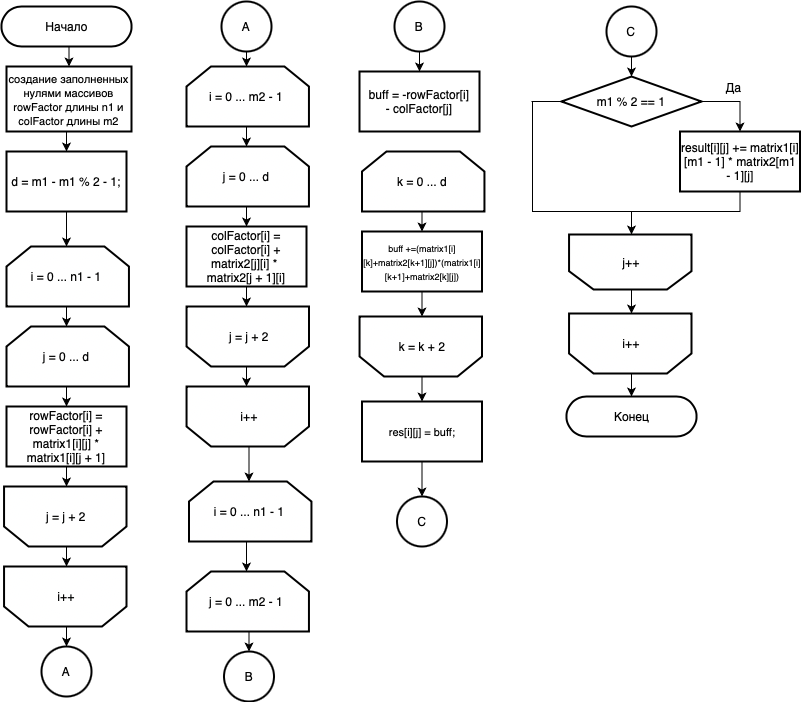
\includegraphics[scale = 0.65]{vinOpt.drawio.png}
	\caption{Схема оптимизированного алгоритма Винограда}
	\label{fig:grapesOpt}
\end{figure}


\section{Модель вычислений}

Для последующего вычисления трудоемкости введём модель вычислений.

\begin{enumerate}
	\item Операции из списка (\ref{for:opers}) имеют трудоемкость 1.
	\begin{equation}
	\label{for:opers}
	+, -, *, /, \%, ==, !=, <, >, <=, >=, [], ++, {-}-
	\end{equation}
	\item Трудоемкость оператора выбора if условие then A else B рассчитывается, как (\ref{for:if}).
	\begin{equation}
	\label{for:if}
	f_{if} = f_{\text{условия}} +
	\begin{cases}
	f_A, & \text{если условие выполняется,}\\
	f_B, & \text{иначе.}
	\end{cases}
	\end{equation}
	\item Трудоемкость цикла рассчитывается, как (\ref{for:for}).
	\begin{equation}
	\label{for:for}
	f_{for} = f_{\text{инициализации}} + f_{\text{сравнения}} + N(f_{\text{тела}} + f_{\text{инкремента}} + f_{\text{сравнения}})
	\end{equation}
	
	где N - количество итераций цикла.
	\item Трудоемкость вызова функции равна 0.
\end{enumerate}

\section{Трудоёмкость алгоритмов}
Примем, что размеры первой матрицы (r, s), второй - (s, c).
\subsection{Стандартный алгоритм умножения матриц}

Трудоёмкость стандартного алгоритма в выбранной модели вычислений в худшем и лучшем случаях рассчитывается следующим образом:
\begin{equation}
	f_{base} = 2 + r(2 + 2 + c(2 + 2 + s(2 + 11))) = 13scr + 4cr + 4r + 2.
\end{equation}

\subsection{Алгоритм Винограда}
Для алгоритма Винограда худшим случаем являются матрицы с нечётным s, а лучшим - с чётным, из-за того что отпадает необходимость в последнем цикле.

Трудоёмкость алгоритма Винограда является суммой трудоёмкостей следующих последовательно выполненных действий.
\begin{enumerate}
	
	\item Заполнения вектора rowFactor:
	\begin{equation}
	f_{rowFactor} = 3 + r(2 + 2 + \frac{s}{2}(2 + 11)) = 6.5sr + 4r + 3.
	\end{equation}
	
	\item Заполнения вектора colFactor:
	\begin{equation}
	f_{colFactor} = 2 + c(2 + 2 + \frac{s}{2}(2 + 11)) = 6.5sc + 4r + 2.
	\end{equation}
	
	\item Основного цикла заполнения матрицы:
	\begin{equation}
	f_{cycle} = 2 + r(2 + 2 + c(2 + 2 + 7 + \frac{s}{2}(2 + 23))) = 12.5scr + 11cr + 4r + 2.
	\end{equation}
	
	\item Цикла для дополнения умножения, если s нечётный:
	\begin{equation}
	f_{last} = \begin{cases}
	2, & \text{s чётный,}\\
	2 + 2 + r(2 + 2 + c(2 + 13)) = 15cr + 4r + 4, & \text{иначе.}
	\end{cases}
	\end{equation}
\end{enumerate}

Итак, для лучшего случая (s чётный): 
\begin{equation}
f_{vin\_b} = 6.5sr + 4r + 3 + 6.5sc + 4r + 2 + 12.5scr + 11cr + 4r + 2 + 2 = 12.5scr + 6.5sr + 6.5sc + 11cr + 12r + 9.
\end{equation}

Для худшего случая (s нечётный): 
\begin{eqnarray}
f_{vin\_w} = 6.5sr + 4r + 3 + 6.5sc + 4r + 2 + 12.5scr + 11cr + 4r + 2 + 15cr + 4r + 4 =\\ = 12.5scr + 6.5sr + 6.5sc + 26cr + 16r + 11.
\end{eqnarray}

\subsection{Оптимизированный алгоритм Винограда}

Трудоёмкость оптимизированного алгоритма Винограда является суммой трудоёмкостей следующих последовательно выполненных действий.
\begin{enumerate}
	\item Заполнения вектора rowFactor:
	\begin{equation}
	f_{rowFactor} = 5 + r(3 + 2 + \frac{s}{2}(3 + 10)) = 6.5sr + 5r + 5.
	\end{equation}
	
	\item Заполнения вектора colFactor:
	\begin{equation}
	f_{colFactor} = 2 + c(2 + 2 + \frac{s}{2}(2 + 11)) = 6.5sс + 5r + 2.
	\end{equation}
	
	\item Основного цикла заполнения матрицы:
	\begin{equation}
	f_{cycle} = 3 + 2 + r(2 + 2 + c(2 + 2 + 5 + \frac{s}{2}(3 + 15) + f_{last} + 3)) = 9scr + 12cr + f_{last}cr + 4r + 5.
	\end{equation}
	\begin{equation}
	f_{last} = \begin{cases}
	0, & \text{s чётный,}\\
	9, & \text{иначе.}
	\end{cases}
	\end{equation}
\end{enumerate}

Итак, для лучшего случая (s чётный): 
\begin{equation}
f_{vinOpt\_b} = 6.5sr + 5r + 5 + 6.5sс + 5r + 2 + 9scr + 12cr + 4r + 5 = 9scr + 6.5sr + 6.5sc + 12cr + 14r + 12.
\end{equation}

Для худшего случая (s нечётный): 
\begin{equation}
f_{vinOpt\_w} = 6.5sr + 5r + 5 + 6.5sс + 5r + 2 + 9scr + 12cr + 9cr + 4r + 5 = 9scr + 6.5sr + 6.5sc + 21cr + 14r + 12.
\end{equation}

\section{Вывод}
	На основе теоретических данных, полученных из аналитического раздела, были построены схемы алгоритмов умножения матриц, оценены их трудоёмкости в лучшем и худшем случаях.

\chapter{Технологическая часть}
В данном разделе приводится реализация алгоритмов, схемы которых были разработаны в конструкторской части. Кроме того, обосновывается выбор технологического стека и проводится тестирование реализованных алгоритмов.
\section{Средства реализации}

В качестве языка программирования был выбран C++ из-за его быстродействия, а среды разработки -- CLion.

\section{Реализация алгоритмов}

В листингах \ref{base_code}, \ref{vin_code} и \ref{vin_opt_code} приведены реализации алгоритмов умножения матриц.
\begin{lstlisting}[label=base_code,caption=Функция обычного алгоритма умножения матриц,language=C++]
Matrix Matrix::convMul(Matrix &matr)
{
    Matrix result(rows, matr.cols);
    for (size_t i = 0; i < rows; i++) {
        for (size_t k = 0; k < matr.cols; k++) {
            result.matrix_ptr[i][k] = 0;
            for (size_t j = 0; j < cols; j++)
                result.matrix_ptr[i][k] += matrix_ptr[i][j] * matr.matrix_ptr[j][k];
        }
    }
    return result;
}
\end{lstlisting}
\newpage
\begin{lstlisting}[label=vin_code,caption=Функция алгоритма умножения матриц Винограда,language=C++]
Matrix Matrix::vinogradMul(Matrix &matr)
{
    Matrix res(rows, matr.cols);
    double *rowFactor = (double *) malloc (rows * sizeof(double));
    double *colFactor = (double *) malloc (matr.cols * sizeof(double ));

    int d = this->cols / 2;
    for (int i = 0; i < this->rows; i++) {
        rowFactor[i] = matrix_ptr[i][0] * matrix_ptr[i][1];
        for (int j = 1; j < d; j++)
        {
            rowFactor[i] = rowFactor[i] + matrix_ptr[i][2 * j] * matrix_ptr[i][2 * j + 1];

        }
    }

    for (int i = 0; i < matr.cols; i++) {
        colFactor[i] = matr.matrix_ptr[0][i] * matr.matrix_ptr[1][i];
        for (int j = 1; j < d; j++)
        {
            colFactor[i] = colFactor[i] + matr.matrix_ptr[2 * j][i] * matr.matrix_ptr[2 * j + 1][i];
        }
    }

    for (int i = 0; i < this->rows; i++) {
        for (int j = 0; j < matr.cols; j++) {
            res.matrix_ptr[i][j] = -rowFactor[i] - colFactor[j];
            for (int k = 0; k < d; k++)
                res.matrix_ptr[i][j] = res.matrix_ptr[i][j] + (matrix_ptr[i][2 * k] + matr.matrix_ptr[2 * k + 1][j]) * (matrix_ptr[i][2 * k + 1] + matr.matrix_ptr[2 * k][j]);
        }
    }

    if (this->cols % 2 == 1)
    {
        for (int i = 0; i < rows; i++)
            for (int j = 0; j < matr.cols; j++)
                res.matrix_ptr[i][j] = res.matrix_ptr[i][j] + matrix_ptr[i][this->cols - 1] * matr.matrix_ptr[this->cols - 1][j];
    }
    free(rowFactor);
    free(colFactor);
    return res;
}
\end{lstlisting}
\newpage
\begin{lstlisting}[label=vin_opt_code,caption=Функция оптимизированного алгоритма умножения матриц Винограда,language=C++]
Matrix Matrix::optimizedMul(Matrix &matr)
{
    Matrix res(rows, matr.cols);
    double *rowFactor = (double *) malloc (rows * sizeof(double));
    double *colFactor = (double *) malloc (matr.cols * sizeof(double ));

    int d = cols - cols % 2;
    for (int i = 0; i < this->rows; ++i, ++i) {
        rowFactor[i] = 0;
        for (int j = 0; j < d; ++j, ++j)
            rowFactor[i] = rowFactor[i] + matrix_ptr[i][j] * matrix_ptr[i][j + 1];
    }

    for (int i = 0; i < matr.cols; i++) {
        colFactor[i] = 0;
        for (int j = 0; j < d; ++j, ++j)
        {
            colFactor[i] = colFactor[i] + matr.matrix_ptr[j][i] * matr.matrix_ptr[j + 1][i];
        }
    }

    bool flag = this->cols % 2 == 1;
    double buf;
    for (int i = 0; i < this->rows; ++i) {
        for (int j = 0; j < matr.cols; ++j) {
            buf = -rowFactor[i] - colFactor[j];
            for (int k = 0; k < d; ++k, ++k)
                buf = buf + (matrix_ptr[i][k] + matr.matrix_ptr[k + 1][j]) *
                                                              (matrix_ptr[i][k + 1] + matr.matrix_ptr[k][j]);
            if (flag)
                buf = buf + matrix_ptr[i][this->cols - 1] * matr.matrix_ptr[this->cols - 1][j];
            res.matrix_ptr[i][j] = buf;
        }
    }
    free(rowFactor);
    free(colFactor);
    return res;
}
\end{lstlisting}

\newpage
\section{Тестирование}

В таблице~\ref{tabular:test_rec} приведены модульные тесты для функций, реализующих стандартный алгоритм умножения матриц, алгоритм Винограда и оптимизированный алгоритм Винограда. Методолгия тестирования - чёрный ящик.

\begin{table}[h!]
	\begin{center}
	\caption{\label{tabular:test_rec} Тестирование функций}
		\begin{tabular}{c@{\hspace{7mm}}c@{\hspace{7mm}}c@{\hspace{7mm}}c@{\hspace{7mm}}c@{\hspace{7mm}}c@{\hspace{7mm}}}
			\hline
			Первая матрица & Вторая матрица & Ожидаемый результат \\ \hline
			\vspace{4mm}
			$\begin{pmatrix}
			1 & 2 & 3\\
            3 & 4 & 5
			\end{pmatrix}$ &
			$\begin{pmatrix}
			2 & 3 & 7\\
            5 & 1 & 10\\
            6 & -1 & 4
			\end{pmatrix}$ &
			$\begin{pmatrix}
			12 & 5 & 27 \\
			26 & 13 & 61 
			\end{pmatrix}$ \\
			\vspace{2mm}
			\vspace{2mm}
			$\begin{pmatrix}
			1 & 2\\
            3 & 4
			\end{pmatrix}$ &
			$\begin{pmatrix}
			2 & 3 & 7\\
            5 & 1 & 10
			\end{pmatrix}$ &
			$\begin{pmatrix}
			12 & 5 & 27 \\
			26 & 13 & 61 
			\end{pmatrix}$ \\
			\vspace{2mm}
			\vspace{2mm}
			$\begin{pmatrix}
			2
			\end{pmatrix}$ &
			$\begin{pmatrix}
			2
			\end{pmatrix}$ &
			$\begin{pmatrix}
			4
			\end{pmatrix}$ \\
			\vspace{2mm}
			\vspace{2mm}
			$\begin{pmatrix}
			1 & -2 & 3\\
			1 & 2 & 3\\
			1 & 2 & 3
			\end{pmatrix}$ &
			$\begin{pmatrix}
			-1 & 2 & 3\\
			1 & 2 & 3\\
			1 & 2 & 3
			\end{pmatrix}$ &
			$\begin{pmatrix}
			0 & 4 & 6\\
			4 & 12 & 18\\
			4 & 12 & 18
			\end{pmatrix}$\\
			\vspace{2mm}
			\vspace{2mm}
		\end{tabular}
	\end{center}
\end{table}
Все тесты пройдены успешно.
\section{Вывод}

В данном разделе были реализованы алгоритмы умножения матриц: обычный алгоритм, алгоритм Винограда и оптимизированный алгоритм Винограда. Кроме того, реализации были успешно протестированы.

\chapter{Исследовательская часть}
В эданном разделе проводится сравнительный анализ реализованных алгоритмов по процессорному времени.
\section{Технические характеристики}

Все нижепреведенные замеры времени проведены на процессоре: Intel Core i5, 1,4 GHz, 4ядерный. Время работы алгоритмов было замерено с помощью time.h, функции clock, которая измеряет процессорное время [1].

\section{Время выполнения реализаций алгоритмов}

Для сравнительного анализа времени выполнения реализаций алгоритмов был проведен эксперимент. Для замеров были сформированы следующие пары матриц.
\begin{enumerate}
	\item Внутренний размер чётный и варьируется в пределах от 1000 до 2100 с шагом 100, а внешний постоянен и равен 100.
	\item Внутренний размер нечётный и варьируется в пределах от 1001 до 2101 с шагом 100, а внешний постоянен и равен 100.
\end{enumerate}

В таблицах \ref{timeEvenTable} и \ref{timeOddTable} представлены результаты замеров. Время измерялось 10 раз для каждой пары матриц, после усреднялось. 

\begin{table} [h!]
	\caption{Таблица времени выполнения (в мс) алгоритмов при чётных размерах}
	\begin{center}
		\begin{tabular}{|c c c c|} 
		\hline
		Размер матрицы & Стандартный & Виноград & Оптимизированный \\  
		\hline
        1000 & 62.86 & 56.38 & 41.96  \\ 
        \hline
        1100 & 63.60 & 48.91 & 47.35  \\ 
        \hline
        1200 & 67.08 & 52.26 & 49.35  \\ 
        \hline
        1300 & 76.38 & 60.68 & 58.20  \\ 
        \hline
        1400 & 83.19 & 65.09 & 62.93  \\ 
        \hline
        1500 & 92.65 & 71.02 & 70.90  \\ 
        \hline
        1600 & 100.19 & 76.75 & 77.12  \\ 
        \hline
        1700 & 111.02 & 94.34 & 82.80  \\ 
        \hline
        1800 & 115.22 & 97.15 & 87.39  \\ 
        \hline
        1900 & 119.39 & 101.51 & 92.23  \\ 
        \hline
        2000 & 134.29 & 102.36 & 99.96  \\ 
        \hline
		\end{tabular}
	\label{timeEvenTable}
	\end{center}
\end{table}

\begin{table} [h!]
	\caption{Таблица времени выполнения (в мс) алгоритмов при нечётных размерах}
	\begin{center}
	\begin{tabular}{|c c c c|} 
		\hline
		Размер матрицы & Стандартный & Виноград & Оптимизированный \\  
		\hline
        1001 & 56.73 & 60.47 & 42.62  \\ 
        \hline
        1101 & 61.71 & 48.64 & 46.49  \\ 
        \hline
        1201 & 68.57 & 53.81 & 51.87  \\ 
        \hline
        1301 & 76.09 & 59.92 & 57.12  \\ 
        \hline
        1401 & 84.76 & 64.74 & 63.88  \\ 
        \hline
        1501 & 90.83 & 70.58 & 68.64  \\ 
        \hline
        1601 & 98.00 & 75.73 & 76.02  \\ 
        \hline
        1701 & 105.49 & 90.68 & 81.28  \\ 
        \hline
        1801 & 113.42 & 96.89 & 87.83  \\ 
        \hline
        1901 & 121.53 & 103.43 & 93.42  \\ 
        \hline
        2001 & 134.73 & 103.37 & 100.57  \\ 
        \hline
	\end{tabular}
	\label{timeOddTable}
\end{center}
\end{table}
\newpage
Время на графиках \ref{timeEvenGraph} и  \ref{timeOddGraph} представлено в милисекундах. 
\newpage
\begin{figure}[h!p]
	\centering
	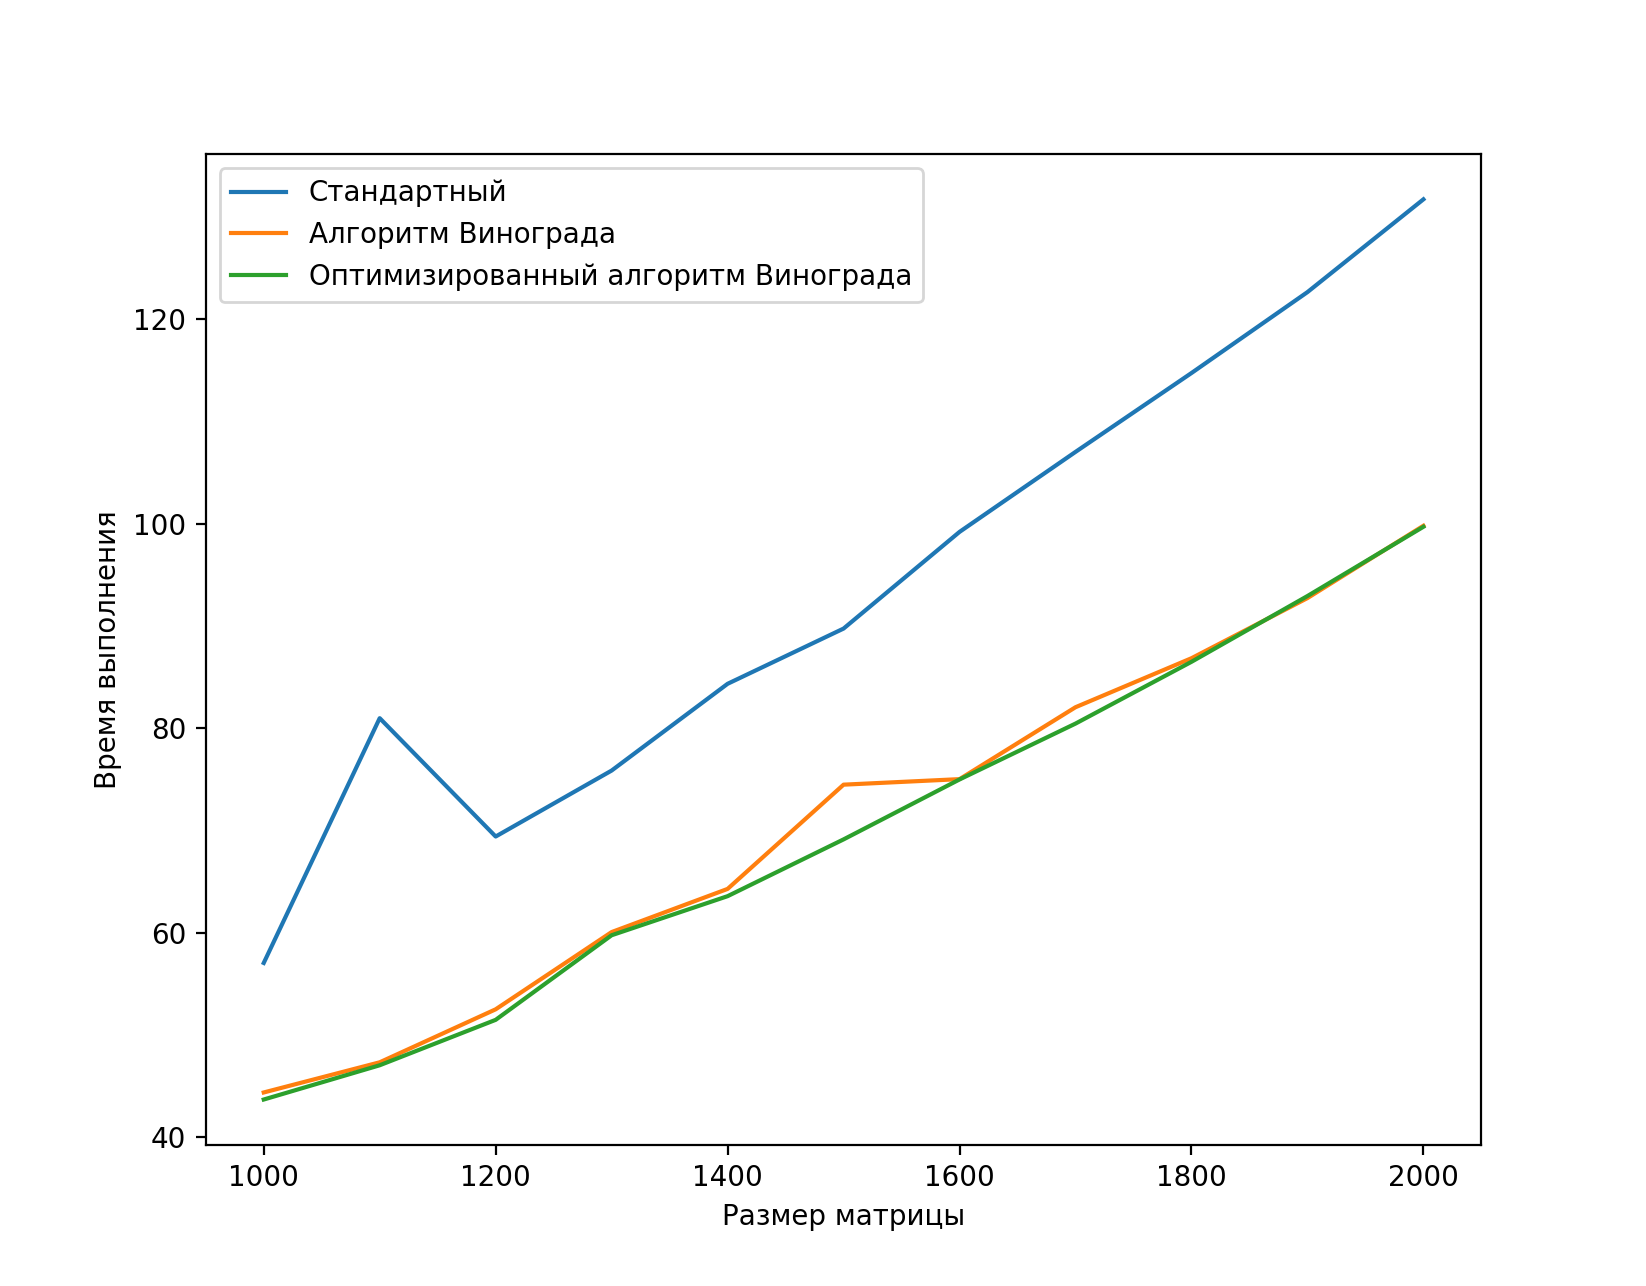
\includegraphics[scale = 0.6]{even.png}
	\caption{Зависимость времени выполнения от размера матриц (чётный)}
	\label{timeEvenGraph}
\end{figure}

\begin{figure}[h!p]
	\centering
	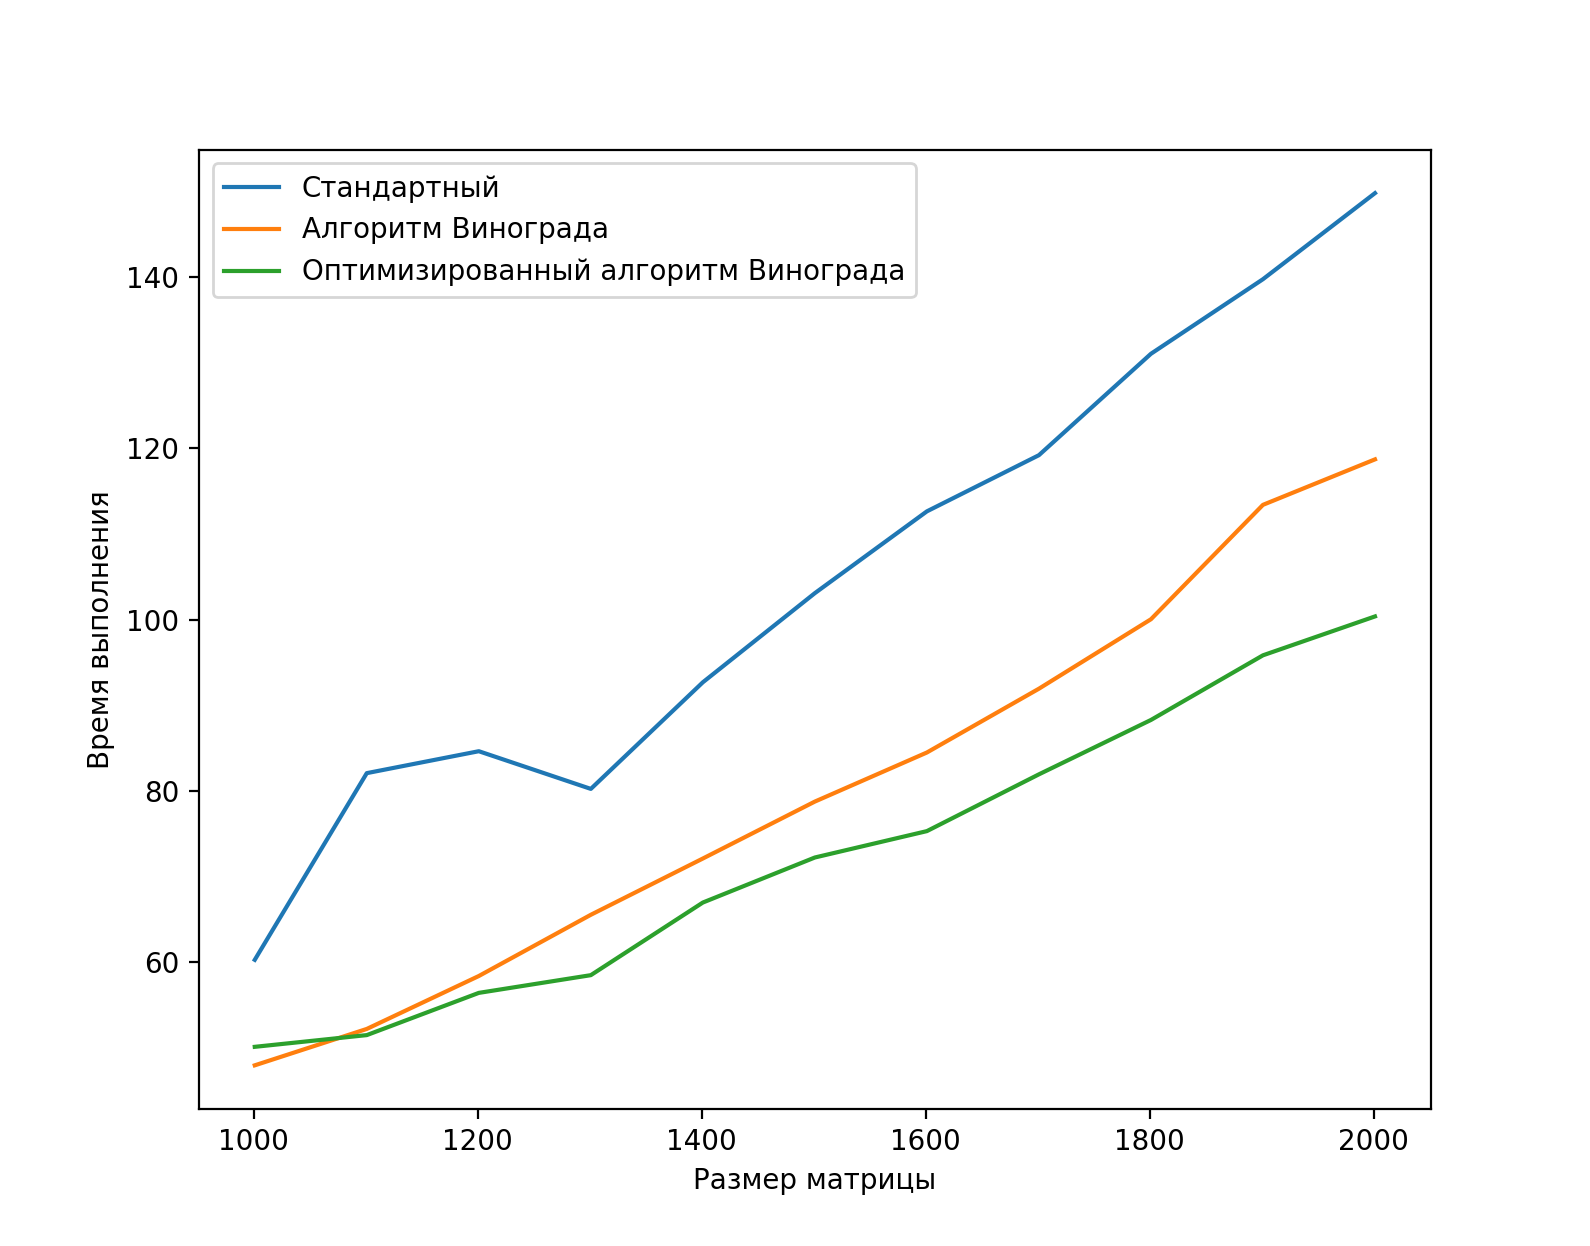
\includegraphics[scale = 0.6]{odd.png}
	\caption{Зависимость времени выполнения от размера матриц (чётный)}
	\label{timeOddGraph}
\end{figure}
\section{Вывод}

На основе замеров процессорного времени было получено, что алгоритм Винограда в среднем в 1.2-1.4 раза быстрее, чем обычный алгоритм умножения матриц и немного хуже оптимизированного.

\chapter*{Заключение}
\addcontentsline{toc}{chapter}{Заключение}

В рамках данной лабораторной работы были решены следующие задачи.
\begin{enumerate}
	\item Были изучены два алгоритма умножения матриц: обычный и алгоритм Винограда.
	\item Разработан оптимизированный алгоритм Винограда.
	\item Реализованы три алгоритма умножения матриц: обычный, алгоритм Винограда и оптимизированный алгоритм Винограда.
	\item Был проведён сравнительный анализ трудоёмкости алгоритмов на основе расчетов в выбранной модели вычислений.
	\item Был проведён равнительный анализ алгоритмов на основе экспериментальных данных.
\end{enumerate}

На основании анализа трудоёмкости алгоритмов в выбранной модели вычислений было показано, что улучшенный алгоритм Винограда имеет меньшую сложность, нежели простой алгоритм умножения матриц. На основании замеров времени исполнения алгоритмов, был сделан вывод о том, что алгоритм Винограда в среднем в 1.2-1.4 раза быстрее, чем обычный алгоритм умножения матриц и немного хуже оптимизированного. 

Поставленная цель была достигнута.

\chapter*{Литература}
\addcontentsline{toc}{chapter}{Литература}
\begin{enumerate}
	\item Стандартная функция clock(), измеряющая процессорное время [Электронный ресурс]. Режим доступа: https://en.cppreference.com/w/cpp/chrono/c/clock. Дата обращения: 03.10.2021
\end{enumerate}

\end{document}